\chapter{Introducción.}\label{sec:introduccion}

%En este capítulo no deben faltar los siguientes apartados:


\section{Motivación del proyecto}

\paragraph{}Hace un año presenté una idea en un concurso de creación de empresas. Mi
idea de empresa estaba basada en el campo de los dispositivos embebidos o IoT. Fue
entonces cuando empecé ha pensar en los desafios tecnológicos que podrían conllevar la
creación de dicha empresa y cómo, estos desafios debían de estar alineados con los
aspectos de negocio.

\paragraph{}Las \glsplural{startup} no siguen las mismas reglas que las empresas tradicionales.
Ésto es debido a que suelen ser empresas concevidas por pocos emprendedores con recursos
limitados, que deben enfrentarse continuamente a cambios y manejar un riesgo alto en
sus decisiones. Por tanto, si una \gls{startup} es de ámbito tecnológico, dicha tecnología tiene
que estar orientada a ser universal y flexible.

\hfill \break

\begin{figure}[ht]
    \centering
    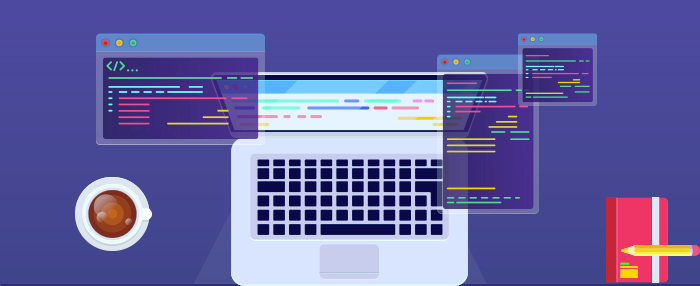
\includegraphics[width=0.65\textwidth]{imgs/dev-env.jpg}
    \caption{Entorno de desarrollo.}
    \label{fig:dev-env}
\end{figure}

\hfill \break

\section{Objetivos}

\paragraph{} Los objetivos de este proyecto se pueden categorizar en objetivos principales,
lo cuales son considerados como esenciales para  definir el éxito del proyecto y
objetivos secundarios que sin ser esenciales nos permiten complementar el análisis,
aprender y sacar conclusiosiones adicionales igualmente valiosas. En conjunto podemos
definir, los siguiente objetivos:

\begin{itemize}
	\item Objetivos Principales
	\begin{itemize}
		\item Diseño e implementación del entorno de desarrollo.
		\item Diseño e implementación del ciclo de vida del desarrollo software.
		\item Explicación del uso del entorno de desarrollo según los roles del equipo
		de desarrolladores.
		\item Diseño e implementación del software de sistema.
		\item Diseño e implementación de una aplicación de meteorología (frontend y backend)
		de características básicas.
		\item Procesos de \textit{testing} y \textit{deployment} de software manuales.
	\end{itemize}
	\item Objetivos Secundarios
	\begin{itemize}
		\item Análisis y justificación de las decisiones tomadas.
		\item Uso de herramientas de código abierto.
		\item Ampliación en las características demostradas con la aplicación de
		meteorología.
		\item Procesos de \textit{testing} y \textit{deployment} de software automátizados.
	\end{itemize}
\end{itemize}


\section{Materiales utilizados}

\paragraph{}Los elementos necesarios para este proyecto son:

\begin{itemize}
	\item Un ordenador de desarrollo.
	\item Ordenador, máquina virtual o servidor de control de versiones.
	\item Ordenador, máquina virtual o servidor de compilaciones.
	\item Una Raspberry Pi conectada a la red local de los desarrolladores.
	\item Pantalla y cable de alimentación de la Raspberry Pi.
\end{itemize}

\section{Estructura del documento}

\paragraph{}A continuación y para facilitar la lectura del documento, se detalla el
contenido de cada capítulo.

\begin{itemize}
\item En el capítulo \ref{sec:introduccion} se realiza una introducción.
\item En el capítulo \ref{sec:estadodelarte} se hace un repaso al estado actual de las
soluciones existentes para abordar las premisas de este proyecto.
\item En el captíulo \ref{sec:EscenarioTrabajo} se presenta al equipo ficticio de
desarrollo, se habla de sus necesidades y de cómo van a interactuar con el entorno.
\item En el capítulo \ref{sec:ManualDeInstalacion} se detallan las instruciones para la
instalación y puesta en marcha del entorno de desarrollo en cada sistema operativo.
\item En el capítulo \ref{sec:GuiaDeUso} se explica las principales herramientas y
opciones presentes en el entorno de desarrollo.
\item En el capítulo \ref{sec:AplicacionMeteorologica} se detallan los aspectos teóricos
de la aplicación de meteorología tales como su interfaz, requisitos y arquitectura.
\item En el capítulo \ref{sec:Desarrollo} se conecta los apartados teóricos de \ref{sec:GuiaDeUso}
y \ref{sec:AplicacionMeteorologica} con la aplicación práctica de los mismos.
\item En el capítulo \ref{sec:cicd} se analíza el ciclo de vida del desarrollo software
y la infraestructura necesaria para llevarlo a cabo.
%\item En el capítulo \ref{sec:}
\item En el capítulo \ref{sec:resultados} se muestran los resultados del proyecto y se
hace un valoración de los mismos.
\item En el capítulo \ref{sec:gestion} se habla de los diferentes recursos utilizados
así como la planificación del proyecto.
\item En el capítulo \ref{sec:conclusiones} se hace una reflexión personal sobre todo
lo relacionado con el proyecto y los aprendizajes extraídos.
\end{itemize}

%las referencias a artículos se ponen con \cite,
%las referencias a glosario \gls,
%y las referencias a ecuaciones \eqref
%las referencias a imgenes, tablas o figuras o secciones
% se ponen con \ref (sólo número) o con \hyperref[sec:X]{text}
